\documentclass[11pt]{article}

\usepackage[a4paper,margin=1in]{geometry}
\usepackage[T1]{fontenc}
\usepackage[utf8]{inputenc}
\usepackage{lmodern}
\usepackage{microtype}
\usepackage{amsmath,amssymb,amsthm,mathtools,mathrsfs}
\usepackage{booktabs,array}
\usepackage{graphicx}
\usepackage{float}
\usepackage[section]{placeins}
\usepackage{enumitem}
\usepackage[numbers,sort&compress]{natbib}
\usepackage{xcolor}
\usepackage{xurl}
\usepackage[colorlinks=true,linkcolor=blue!55!black,citecolor=blue!55!black,urlcolor=blue!55!black]{hyperref}
\usepackage[nameinlink,noabbrev]{cleveref}

\setlength{\parindent}{1.4em}
\setlength{\parskip}{0.12em}
\setlist{itemsep=0.25em,topsep=0.35em}

\newtheorem{theorem}{Theorem}[section]
\newtheorem{proposition}[theorem]{Proposition}
\newtheorem{lemma}[theorem]{Lemma}
\newtheorem{corollary}[theorem]{Corollary}
\theoremstyle{definition}
\newtheorem{definition}[theorem]{Definition}
\theoremstyle{remark}
\newtheorem{remark}[theorem]{Remark}

\newcommand{\R}{\mathbb R}
\newcommand{\C}{\mathbb C}
\newcommand{\Id}{\mathrm I}
\newcommand{\cK}{\mathcal K}
\newcommand{\cB}{\mathcal B}
\newcommand{\cP}{\mathcal P}
\newcommand{\cQ}{\mathcal Q}
\newcommand{\cD}{\mathcal D}
\newcommand{\cS}{\mathfrak S}
\newcommand{\uc}{u_{\mathrm c}}
\newcommand{\norm}[1]{\left\lVert #1\right\rVert}
\newcommand{\tr}{\operatorname{tr}}
\newcommand{\spec}{\operatorname{spec}}
\newcommand{\rank}{\operatorname{rank}}
\newcommand{\detF}{\operatorname{det}}
\newcommand{\Dettwo}{\operatorname{det}\nolimits_2}

\title{A Trace-Ideal Completion of the Intrinsic Bulk Two-Step Operator\\
\large Hilbert--Schmidt Convergence, Trace-Norm Squares, and Fredholm Determinants}
\author{Liang Wang}
\date{July 2026}

\begin{document}
\maketitle

\begin{abstract}
An intrinsic rank-two subtraction has isolated the Perron and negative
parity modes of a folded-Gaussian Markov operator at fixed noise
$\sigma=10^{-2}$.  The resulting bulk operator
\[
 \cB=\cK-\cQ_+-\cQ_-
\]
is the natural one-step complement, but convergence of ordinary Fredholm
determinants would require trace-norm control that is not supplied by the
piecewise-constant discretization.  We close the trace-ideal gap by passing
to the intrinsic two-step operator.

For the full exact-real midpoint family and the adaptive Gaussian-cutoff
family, lifted to $L^2([0,1])$, we prove
\[
 \norm{B_n-\cB}_{\mathfrak S_2}=O(n^{-1}).
\]
Since products of two Hilbert--Schmidt operators are trace class,
\[
 \norm{B_n^2-\cB^2}_{\mathfrak S_1}
 \le \norm{B_n-\cB}_{\mathfrak S_2}
     \bigl(\norm{B_n}_{\mathfrak S_2}
           +\norm{\cB}_{\mathfrak S_2}\bigr)
 =O(n^{-1}).
\]
Consequently every fixed even bulk trace converges, and the Fredholm
determinants
\[
 \cD_{n,\mathrm{bulk}}(w)=\detF(\Id-wB_n^2)
\]
converge locally uniformly on the entire $w$-plane to
$\cD_{\mathrm{bulk}}(w)=\detF(\Id-w\cB^2)$.  The construction is exactly
the symmetric completion of the regularized one-step determinant:
\[
 \Dettwo(\Id-z\cB)\Dettwo(\Id+z\cB)
 =\detF(\Id-z^2\cB^2).
\]

The validated continuum bound is
$\norm{\cB}_{\mathfrak S_2}\le15.418003788081082$.  At $n=65536$ the
outward bounds are $0.1281382922864061$ in Hilbert--Schmidt norm and
$3.967692773690177$ in square trace norm.  At $n=2^{30}$ they decrease to
$3.785070933298939\times10^{-6}$ and
$1.167164903022793\times10^{-4}$; on $|w|\le10^{-2}$ the corresponding
uniform determinant error is at most
$3.682918268863141\times10^{-4}$.  A separate floating sparse-LU pilot at
$2048$, $4096$, and $8192$ shows a mean dyadic determinant-difference ratio
$0.2493$, but this sharper center behavior is not used in the theorem.

All results are at fixed positive noise.  No zero-noise limit, arithmetic
trace formula, prime-power identity, zeta-zero correspondence,
self-adjoint Hilbert--P\'olya operator, or Riemann-hypothesis conclusion is
asserted.
\end{abstract}

\noindent\textbf{Keywords:} Hilbert--Schmidt operator; trace ideal;
Fredholm determinant; regularized determinant; Riesz projection; Markov
operator; Nystr\"om approximation.

\medskip
\noindent\textbf{MSC 2020:} 47B10; 47A10; 65R20; 37M25; 60J05.

\section{Introduction}
\label{sec:introduction}

The useful spectral object in a noisy dynamical system is often not the
full transfer operator but the complement left after isolated peripheral
modes have been removed.  For the folded-Gaussian Markov operator studied
in this series, the Perron eigenvalue $1$ and a simple negative resonance
near $-1$ have now been isolated by explicit Euclidean contours.  Their
weighted Riesz terms are intrinsic, real, smooth, and gauge-free.  Thus the
one-step bulk operator
\begin{equation}
 \cB=\cK-\cQ_+-\cQ_-
 \label{eq:bulk-intro}
\end{equation}
is no longer a numerical ansatz: it is a rigorously defined continuum
operator with validated full and sparse discretizations
\citep{WangParityKernel2026,WangRankTwo2026}.

That completion leaves a trace-ideal mismatch.  The most natural
cellwise comparison is Hilbert--Schmidt.  If $k_n$ is a piecewise-constant
kernel approximation to a smooth kernel $k$, then
\[
 \norm{k_n-k}_{L^2([0,1]^2)}=O(n^{-1})
\]
without requiring pointwise interpolation.  Under the standard isometry
between matrices and piecewise-constant integral operators, this is exactly
Hilbert--Schmidt convergence.  It does not by itself imply trace-norm
convergence.  Therefore one cannot simply pass from
$B_n\to\cB$ in $\mathfrak S_2$ to local uniform convergence of
$\detF(\Id-zB_n)$.

The two-step operator has the missing regularity automatically.  The trace
ideal product rule
\[
 \mathfrak S_2\mathfrak S_2\subset\mathfrak S_1
\]
turns the elementary factorization
\[
 B_n^2-\cB^2=(B_n-\cB)B_n+\cB(B_n-\cB)
\]
into a trace-norm estimate.  This is the central mechanism of the paper.
It is abstract, short, and independent of normality or self-adjointness.
All dynamical work enters through the explicit Hilbert--Schmidt error
ledger for $B_n-\cB$.

There are three reasons that the squared determinant is the correct next
object.
\begin{enumerate}[leftmargin=2em]
 \item It is intrinsic.  Both peripheral branches have already been
 removed by weighted Riesz calculus; no ordering or normalization of
 eigenvectors remains in the definition.
 \item It is trace class under exactly the topology delivered by the
 discretization.  No unproved trace-norm approximation of the one-step
 operator is inserted.
 \item It joins the regularized determinant of the long-cycle analysis by
 the exact identity
 \[
  \Dettwo(\Id-z\cB)\Dettwo(\Id+z\cB)
  =\detF(\Id-z^2\cB^2).
 \]
 The linear regularization terms cancel between $z$ and $-z$.
\end{enumerate}

The distinction between these statements and a Hilbert--P\'olya
construction is substantial.  The operator $\cB$ is nonnormal, the
determinant is attached to one fixed positive noise width, and no arithmetic
trace formula is available.  Squaring packages the even spectral traces; it
does not make the operator self-adjoint and it does not identify any
determinant zero with a Riemann zero.  The result established here is a
functional-analytic bridge needed before such comparisons can even be
formulated cleanly.

\subsection*{Main contribution and evidence levels}

The paper keeps three logical layers separate.
\begin{description}[leftmargin=3.2cm,style=nextline]
 \item[Analytic theorem]
 Hilbert--Schmidt-to-trace-norm squaring, even-trace convergence, Fredholm
 determinant continuity, and the symmetric $\det_2$ identity.
 \item[Outward certificate]
 Explicit continuum kernel bounds, Hilbert--Galerkin errors, midpoint and
 row-normalization errors, adaptive Gaussian-cutoff errors, and
 Perron/parity weighted-Riesz transport for every $n\ge65536$.
 \item[Floating diagnostic]
 Sparse-LU determinant values for the exact archived binary64 matrices at
 $2048$, $4096$, and $8192$.  These values illustrate stabilization but
 prove no continuum statement.
\end{description}

\section{Operator, contours, and discretizations}
\label{sec:operator}

Let $\uc$ be the unique root in $(1.5,1.6)$ of
\[
 u^3-2u^2+2u-2=0,
\]
fix $\sigma=1/100$, and put
\[
 m(x)=1-\uc x^2.
\]
For $x,y\in[0,1]$, define
\begin{align}
 g(x,y)&=
 e^{-(y-m(x))^2/(2\sigma^2)}
 +e^{-(y+m(x))^2/(2\sigma^2)},
 \label{eq:g-kernel}\\
 Z(x)&=\int_0^1g(x,y)\,dy,
 \qquad
 k(x,y)=\frac{g(x,y)}{Z(x)}.
 \label{eq:normalized-kernel}
\end{align}
The folded Markov operator on $H=L^2([0,1])$ is
\begin{equation}
 (\cK f)(x)=\int_0^1k(x,y)f(y)\,dy.
 \label{eq:markov-operator}
\end{equation}
Its kernel is real, strictly positive, and smooth on the compact square,
and $\cK\mathbf1=\mathbf1$.

The validated contours are
\begin{align}
 \Gamma_+&=\{z\in\C:|z-1|=0.05\},
 \label{eq:perron-contour}\\
 \Gamma_-&=\{z\in\C:|z+0.9865481927458079|=0.05\}.
 \label{eq:parity-contour}
\end{align}
Each contains one algebraically simple eigenvalue, and the circles are
disjoint.  Their weighted Riesz terms are
\begin{equation}
 \cQ_\pm
 =\frac{1}{2\pi i}\int_{\Gamma_\pm}
 z(z-\cK)^{-1}\,dz.
 \label{eq:weighted-riesz}
\end{equation}
For the Perron branch, $\cQ_+$ is also the rank-one projection
$f\mapsto\mathbf1\langle\pi,f\rangle$, where
$\cK^*\pi=\pi$ and $\int_0^1\pi=1$.  For the negative branch,
$\cQ_-=\lambda_-\cP_-$, where $\cP_-$ is its Riesz projection.  The
terms commute with $\cK$, annihilate one another, and have smooth real
rank-one kernels.  We use the bulk definition \eqref{eq:bulk-intro}.

\subsection{Cell spaces and lifted matrices}

Let $I_{n,j}=[j/n,(j+1)/n)$ and let $V_n\subset H$ be the space of
functions constant on the $n$ cells.  The vectors
\[
 e_{n,j}=\sqrt n\,\mathbf1_{I_{n,j}},
 \qquad 0\le j<n,
\]
form an orthonormal basis.  Write $E_n$ for the orthogonal projection onto
$V_n$ and $J_n:\C^n\to V_n$ for the corresponding isometry.  Every matrix
$A_n$ is compared with the continuum through the zero-complement lift
\begin{equation}
 \widehat A_n=J_nA_nJ_n^*.
 \label{eq:matrix-lift}
\end{equation}
Then
\[
 \norm{\widehat A_n}_{\mathfrak S_2}=\norm{A_n}_{\mathrm F}.
\]
We suppress the hat after this convention has been fixed.

Let $x_i=y_i=(i+\tfrac12)/n$ and $h=1/n$.  The continuum-normalized
midpoint matrix is
\begin{equation}
 (P_n^\circ)_{ij}=h k(x_i,y_j).
 \label{eq:midpoint-matrix}
\end{equation}
The full exact-real matrix $P_n$ row-normalizes the unnormalized folded
Gaussian midpoint weights.  The adaptive matrix $P_n^{\mathrm{ad}}$ first
retains destinations within $L_n\sigma$ of either folded mean and then
renormalizes, where
\begin{equation}
 L_n=\max\{8,2\sqrt{\log n}\}.
 \label{eq:adaptive-schedule}
\end{equation}
At $n=2048,4096,8192$, one has $L_n=8$, so the archived fixed-width
matrices are also exact members of the declared adaptive sequence.

For $F_n\in\{P_n,P_n^{\mathrm{ad}}\}$, define
\begin{equation}
 Q_{\pm,n}
 =\frac{1}{2\pi i}\int_{\Gamma_\pm}
 z(z-F_n)^{-1}\,dz,
 \qquad
 B_n=F_n-Q_{+,n}-Q_{-,n}.
 \label{eq:discrete-bulk}
\end{equation}
The all-grid contour theorem of the preceding work makes these definitions
valid for every integer $n\ge65536$.

\section{The abstract trace-ideal mechanism}
\label{sec:abstract}

We write $\mathfrak S_2(H)$ and $\mathfrak S_1(H)$ for the
Hilbert--Schmidt and trace-class ideals.  Their norms are denoted by
$\norm{\cdot}_2$ and $\norm{\cdot}_1$ in this section.

\begin{lemma}[Hilbert--Schmidt square continuity]
\label{lem:square-continuity}
If $X,Y\in\mathfrak S_2(H)$, then $X^2,Y^2\in\mathfrak S_1(H)$ and
\begin{equation}
 \norm{X^2-Y^2}_1
 \le \norm{X-Y}_2\bigl(\norm X_2+\norm Y_2\bigr).
 \label{eq:square-continuity}
\end{equation}
\end{lemma}

\begin{proof}
Use
\[
 X^2-Y^2=(X-Y)X+Y(X-Y)
\]
and the ideal inequality
$\norm{AC}_1\le\norm A_2\norm C_2$ for
$A,C\in\mathfrak S_2(H)$ \citep{Simon2005,GohbergKrein1969}.
\end{proof}

\begin{theorem}[Squares, even traces, and determinants]
\label{thm:abstract}
Suppose $B_n,B\in\mathfrak S_2(H)$ and
\begin{equation}
 \norm{B_n-B}_2\le\varepsilon_n,
 \qquad
 \norm B_2\le M.
 \label{eq:abstract-hs-input}
\end{equation}
Put
\begin{equation}
 \delta_n=\varepsilon_n(2M+\varepsilon_n).
 \label{eq:delta-definition}
\end{equation}
Then
\begin{align}
 \norm{B^2}_1&\le M^2,
 \label{eq:continuum-square-trace-upper}\\
 \norm{B_n^2}_1&\le(M+\varepsilon_n)^2,
 \label{eq:discrete-square-trace-upper}\\
 \norm{B_n^2-B^2}_1&\le\delta_n.
 \label{eq:trace-norm-square-error}
\end{align}
For every fixed integer $m\ge1$,
\begin{equation}
 \left|\tr(B_n^{2m})-\tr(B^{2m})\right|
 \le m\delta_n
 \left[\max\{M^2,(M+\varepsilon_n)^2\}\right]^{m-1}.
 \label{eq:even-trace-error}
\end{equation}
Moreover, with
\begin{equation}
 \cD_n(w)=\detF(\Id-wB_n^2),
 \qquad
 \cD(w)=\detF(\Id-wB^2),
 \label{eq:determinants-defined}
\end{equation}
one has, for every $R\ge0$,
\begin{equation}
 \sup_{|w|\le R}|\cD_n(w)-\cD(w)|
 \le R\delta_n
 \exp\!\left(1+RM^2+R(M+\varepsilon_n)^2\right).
 \label{eq:determinant-disk-bound}
\end{equation}
In particular, $\varepsilon_n\to0$ implies local uniform convergence
$\cD_n\to\cD$ on $\C$.
\end{theorem}

\begin{proof}
The first three bounds follow from
$\norm{AC}_1\le\norm A_2\norm C_2$, the triangle inequality, and
\cref{lem:square-continuity}.  For traces, put $A_n=B_n^2$ and $A=B^2$.
The telescoping identity
\[
 A_n^m-A^m
 =\sum_{j=0}^{m-1}A_n^j(A_n-A)A^{m-1-j}
\]
and $\norm{RST}_1\le\norm R\,\norm S_1\,\norm T$ give
\[
 \norm{A_n^m-A^m}_1
 \le m\norm{A_n-A}_1
 \max\{\norm{A_n},\norm A\}^{m-1}.
\]
Use $\norm A\le\norm A_1$ and
$|\tr C|\le\norm C_1$.

For determinants, the standard trace-ideal continuity estimate is
\begin{equation}
 |\detF(\Id+C)-\detF(\Id+D)|
 \le\norm{C-D}_1
 e^{1+\norm C_1+\norm D_1}
 \label{eq:standard-determinant-bound}
\end{equation}
for trace-class $C,D$ \citep{Simon2005}.  Apply it to
$C=-wB_n^2$ and $D=-wB^2$, then maximize over $|w|\le R$.
\end{proof}

\begin{remark}[Why the one-step determinant is not used]
\label{rem:one-step-boundary}
At the fixed smooth Gaussian kernel, stronger trace-class regularity of
$\cB$ is available.  What is not supplied by the present discretization
ledger is convergence $B_n\to\cB$ in trace norm.  The theorem therefore
does not infer convergence of $\detF(\Id-zB_n)$ from
Hilbert--Schmidt convergence.  Passing to $B_n^2$ is the rigorously
justified trace-ideal completion.
\end{remark}

\section{Hilbert--Schmidt convergence of the intrinsic bulk}
\label{sec:hs-convergence}

The dynamical part of the argument is to construct an explicit
$\varepsilon_n$ in \eqref{eq:abstract-hs-input}.  It has a Markov-kernel
part and two weighted-Riesz parts.

\subsection{Continuum to cell-average Galerkin}

Let $k_n^{\mathrm G}$ be the kernel of $E_n\cK E_n$.  Applying the
cellwise Poincar\'e--Wirtinger inequality in the source and target variables
gives
\begin{equation}
 \norm{\cK-E_n\cK E_n}_{\mathfrak S_2}
 =\norm{k-k_n^{\mathrm G}}_{L^2([0,1]^2)}
 \le\frac{1}{\pi n}
 \left(\norm{k_x}_{L^2}+\norm{k_y}_{L^2}\right).
 \label{eq:hs-galerkin}
\end{equation}
This first-order term is the asymptotic bottleneck of the current proof.
It is the natural price of lifting a smooth kernel by cell constants rather
than a higher-order basis.

\subsection{Midpoint and exact row normalization}

The one-dimensional midpoint-average Peano kernel has $L^2$ norm
$h^{3/2}/\sqrt{320}$.  Tensor decomposition therefore gives
\begin{equation}
 \norm{E_n\cK E_n-P_n^\circ}_{\mathfrak S_2}
 \le \frac{h^2}{\sqrt{320}}
 \left(\norm{k_{xx}}_{L^2}+\norm{k_{yy}}_{L^2}\right)
 +\frac{h^4}{320}\norm{k_{xxyy}}_{L^2}.
 \label{eq:midpoint-hs}
\end{equation}

Let $Z_*>0$ be the validated normalizer lower bound and put
\begin{equation}
 a_n=\frac{e^{-1/2}}{\sigma}h^2,
 \qquad
 \rho_n=\frac{a_n}{Z_*-a_n}.
 \label{eq:normalization-scaling}
\end{equation}
Exact row normalization is a diagonal left scaling whose relative defect is
at most $\rho_n$.  Hence
\begin{equation}
 \norm{P_n-P_n^\circ}_{\mathfrak S_2}
 \le \rho_n
 \left(\norm k_{L^2}+\norm{E_n\cK E_n-P_n^\circ}_{\mathfrak S_2}\right).
 \label{eq:normalization-hs}
\end{equation}
Although the inherited certificate field was originally named
``spectral norm defect,'' its derivation is a relative row-scaling bound
times a Frobenius kernel norm.  It is therefore also a valid
Hilbert--Schmidt upper bound.

\subsection{Adaptive Gaussian cutoff}

For a declared support multiple $L$, the omitted row mass obeys
\begin{equation}
 \mu_{n,L}
 \le
 \frac{2\sqrt e\,e^{-L^2/2}(h+\sigma/L)}{\sigma-h}.
 \label{eq:cutoff-mass}
\end{equation}
Writing $\alpha_{n,L}=\mu_{n,L}/(1-\mu_{n,L})$, the omitted and
renormalization terms give the Frobenius-square ledger
\begin{align}
 \norm{P_n^{(L)}-P_n}_{\mathfrak S_2}^2
 \le{}&
 \frac{4e\,e^{-L^2}(h+\sigma/(2L))}{(\sigma-h)^2}
 \notag\\
 &+\frac{e\alpha_{n,L}^2(4h+2\sqrt\pi\sigma)}{(\sigma-h)^2}.
 \label{eq:cutoff-hs}
\end{align}
Thus \eqref{eq:adaptive-schedule} gives
\begin{equation}
 \norm{P_n^{\mathrm{ad}}-P_n}_{\mathfrak S_2}
 =O\!\left(n^{-2}(\log n)^{-1/4}\right).
 \label{eq:adaptive-cutoff-rate}
\end{equation}
The certificate field for \eqref{eq:cutoff-hs} is also historically named
``spectral norm upper,'' but it is explicitly the square root of a
Frobenius-square ledger and may be used in $\mathfrak S_2$.

\subsection{Weighted-Riesz transport}

For a circle $\Gamma$ of radius $r$, with
$R_\Gamma=\max_{z\in\Gamma}|z|$, the resolvent identity gives
\begin{equation}
 \norm{\cQ(A;\Gamma)-\cQ(C;\Gamma)}
 \le rR_\Gamma M_A M_C\norm{A-C},
 \label{eq:weighted-lipschitz}
\end{equation}
provided the two contour resolvents are bounded by $M_A$ and $M_C$.
The validated continuum bounds are
\begin{equation}
 \sup_{\Gamma_+}\norm{(z-\cK)^{-1}}
 \le81.30575843422578,
 \qquad
 \sup_{\Gamma_-}\norm{(z-\cK)^{-1}}
 \le112.95503061584434.
 \label{eq:continuum-resolvents}
\end{equation}

The comparison between the continuum weighted term and its Galerkin
compression uses the orthogonal splitting $H=V_n\oplus V_n^\perp$.  The
source-to-detail and target-to-detail blocks are $O(n^{-1})$, while the
detail block is $O(n^{-2})$.  Schur inversion leaves four weighted
resolvent blocks.  In particular, the top-left Schur inverse is the
$V_n$ compression of the complete continuum resolvent, so its norm is at
most the corresponding bound in \eqref{eq:continuum-resolvents}.  This is
the reason the certificate may use the continuum resolvent as the
``Schur-inverse upper.''

Let $\eta_{\pm,n}$ denote the complete operator-norm weighted-term error
after the complement Schur transport, midpoint transfer, exact
normalization, and, when applicable, adaptive cutoff.  Since both the
continuum and discrete weighted terms have rank one,
\begin{equation}
 \rank(Q_{\pm,n}-\cQ_\pm)\le2,
 \qquad
 \norm{Q_{\pm,n}-\cQ_\pm}_{\mathfrak S_2}
 \le\sqrt2\,\eta_{\pm,n}.
 \label{eq:rank-two-hs-conversion}
\end{equation}
All transferred contour gates are closed at $n=65536$.  Every input defect
decreases with $n$, and $L_n$ is nondecreasing, so the same is true for
every integer $n\ge65536$.

\begin{theorem}[Validated bulk Hilbert--Schmidt convergence]
\label{thm:bulk-hs}
For the full and adaptive families in \eqref{eq:discrete-bulk}, and every
integer $n\ge65536$, there are explicit outward numbers
$\varepsilon_n^{\mathrm{full}}$ and
$\varepsilon_n^{\mathrm{ad}}$ such that
\begin{align}
 \norm{B_n^{\mathrm{full}}-\cB}_{\mathfrak S_2}
 &\le\varepsilon_n^{\mathrm{full}}=O(n^{-1}),
 \label{eq:full-hs-rate}\\
 \norm{B_n^{\mathrm{ad}}-\cB}_{\mathfrak S_2}
 &\le\varepsilon_n^{\mathrm{ad}}=O(n^{-1}).
 \label{eq:adaptive-hs-rate}
\end{align}
They are composed as
\begin{equation}
 \varepsilon_n
 =\eta_{K,n}+\sqrt2(\eta_{+,n}+\eta_{-,n}),
 \label{eq:bulk-ledger-composition}
\end{equation}
where $\eta_{K,n}$ is the appropriate full or adaptive Markov
Hilbert--Schmidt defect.

The intrinsic continuum bulk satisfies
\begin{equation}
 \norm{\cB}_{\mathfrak S_2}
 \le \norm{\cK}_{\mathfrak S_2}
     +\norm{\cQ_++\cQ_-}_{\mathfrak S_2}
 \le15.418003788081082.
 \label{eq:bulk-hs-upper}
\end{equation}
\end{theorem}

\begin{proof}
Add \eqref{eq:hs-galerkin}, \eqref{eq:midpoint-hs}, and
\eqref{eq:normalization-hs}, together with \eqref{eq:cutoff-hs} for the
adaptive family.  Add the two weighted-term errors using
\eqref{eq:rank-two-hs-conversion}.  The first-order terms are the cellwise
Galerkin defect and the continuum-complement weighted transport; all other
terms are second order or smaller.  The final continuum bound uses the
validated values
\[
 \norm{\cK}_{\mathfrak S_2}\le5.498549224049743,
 \qquad
 \norm{\cQ_++\cQ_-}_{\mathfrak S_2}
 \le9.919454564031339.
\]
\end{proof}

\begin{remark}[Fixed eight-sigma support]
The fixed-width family remains uniformly spectrally stable and its
peripheral terms are well defined.  Its omitted Gaussian mass has a
nonzero continuum floor, so this paper does not claim that the fixed
eight-sigma family converges to $\cB$ in Hilbert--Schmidt norm.  Adaptive
growth is essential to the continuum theorem.
\end{remark}

\section{Trace-norm squares and even bulk traces}
\label{sec:trace-norm}

Combining \cref{thm:abstract,thm:bulk-hs} immediately closes the
two-step trace ideal.

\begin{theorem}[Validated bulk-square trace-norm convergence]
\label{thm:bulk-square}
For the full and adaptive families, every integer $n\ge65536$ satisfies
\begin{equation}
 \norm{(B_n^{\star})^2-\cB^2}_{\mathfrak S_1}
 \le\delta_n^{\star}
 :=\varepsilon_n^{\star}
 \left(30.836007576162164+\varepsilon_n^{\star}\right),
 \qquad
 \star\in\{\mathrm{full},\mathrm{ad}\}.
 \label{eq:validated-trace-norm}
\end{equation}
In particular,
\begin{equation}
 \norm{(B_n^{\star})^2-\cB^2}_{\mathfrak S_1}=O(n^{-1}).
 \label{eq:trace-norm-rate}
\end{equation}
For every fixed $m\ge1$,
\begin{equation}
 \tr\!\left((B_n^{\star})^{2m}\right)
 \longrightarrow\tr(\cB^{2m}).
 \label{eq:even-trace-convergence}
\end{equation}
The explicit coefficient error is \eqref{eq:even-trace-error} with
$M=15.418003788081082$ and
$\varepsilon_n=\varepsilon_n^\star$.
\end{theorem}

The result is stronger than convergence of a finite list of computed
eigenvalues.  Trace-norm convergence controls the complete compact spectrum
of the two-step operator at the level needed by Fredholm determinants.  It
also controls each even trace without a spectral diagonalization and
without assuming normality.

At the threshold $n=65536$, the full ledger decomposes as
\begin{align}
 \eta_{K,n}&\le0.005119125317796473,
 \notag\\
 \eta_{+,n}&\le0.026770586570540194,
 \qquad
 \eta_{-,n}\le0.06021710060888367,
 \label{eq:threshold-components}\\
 \sqrt2(\eta_{+,n}+\eta_{-,n})
 &\le0.12301916696860951.
 \notag
\end{align}
Thus
\[
 \varepsilon_{65536}^{\mathrm{full}}
 \le0.1281382922864061,
 \qquad
 \delta_{65536}^{\mathrm{full}}
 \le3.967692773690177.
\]
The threshold constants are intentionally conservative: their purpose is
to certify the topology and the asymptotic convergence, not to approximate
the determinant sharply at the smallest admitted grid.

\begin{table}[H]
\centering
\small
\begin{tabular}{rrrrrr}
\toprule
$n$ & $\varepsilon_n^{\rm full}$ & $\varepsilon_n^{\rm ad}$
& $\delta_n^{\rm full}$
& $\Delta_n(10^{-3})$ & $\Delta_n(10^{-2})$\\
\midrule
$2^{16}$
& $1.2814\times10^{-1}$ & $1.2814\times10^{-1}$
& $3.9677$ & $1.7419\times10^{-2}$ & $1.3027\times10^{1}$\\
$2^{20}$
& $3.9318\times10^{-3}$ & $3.9318\times10^{-3}$
& $1.2126\times10^{-1}$ & $5.3031\times10^{-4}$ & $3.8309\times10^{-1}$\\
$2^{24}$
& $2.4245\times10^{-4}$ & $2.4245\times10^{-4}$
& $7.4761\times10^{-3}$ & $3.2693\times10^{-5}$ & $2.3592\times10^{-2}$\\
$2^{30}$
& $3.7851\times10^{-6}$ & $3.7851\times10^{-6}$
& $1.1672\times10^{-4}$ & $5.1039\times10^{-7}$ & $3.6829\times10^{-4}$\\
\bottomrule
\end{tabular}
\caption{Selected outward ledgers.  Here $\varepsilon_n$ is the bulk
Hilbert--Schmidt error, $\delta_n$ is the bulk-square trace-norm error, and
$\Delta_n(R)$ is the full-family determinant upper on $|w|\le R$ from
\eqref{eq:determinant-disk-bound}.  Full and adaptive values agree to the
displayed precision because the adaptive cutoff is much smaller than the
first-order Galerkin term.}
\label{tab:certificate}
\end{table}

The scaled final values are
\begin{equation}
 2^{30}\varepsilon_{2^{30}}^{\mathrm{full}}
 \le4064.188967889787,
 \qquad
 2^{30}\delta_{2^{30}}^{\mathrm{full}}
 \le125323.3771880477.
 \label{eq:scaled-final}
\end{equation}
They exhibit the certified first-order regime.  The constants are larger at
$2^{16}$ because the contour-resolvent transfers have not yet reached their
asymptotic values.

\section{Fredholm determinants and the symmetric regularization identity}
\label{sec:determinants}

Since $\cB^2\in\mathfrak S_1$, define the intrinsic bulk two-step
determinant
\begin{equation}
 \cD_{\mathrm{bulk}}(w)
 =\detF(\Id-w\cB^2).
 \label{eq:bulk-square-determinant}
\end{equation}
It is entire in $w$.  In the norm-safe disk
$|w|\norm{\cB^2}<1$, its logarithm has the trace expansion
\begin{equation}
 \log\cD_{\mathrm{bulk}}(w)
 =-\sum_{m\ge1}\frac{w^m}{m}\tr(\cB^{2m}).
 \label{eq:bulk-square-trace-series}
\end{equation}
Thus the coefficients are precisely the even intrinsic bulk traces closed
in \cref{thm:bulk-square}.

\begin{theorem}[Locally uniform determinant convergence]
\label{thm:determinant-convergence}
For $\star\in\{\mathrm{full},\mathrm{ad}\}$, put
\begin{equation}
 \cD_{n,\mathrm{bulk}}^\star(w)
 =\detF\!\left(\Id-w(B_n^\star)^2\right).
 \label{eq:discrete-square-determinant}
\end{equation}
Then
\begin{equation}
 \cD_{n,\mathrm{bulk}}^\star
 \longrightarrow\cD_{\mathrm{bulk}}
 \quad\text{locally uniformly on }\C.
 \label{eq:local-uniform}
\end{equation}
For every $R\ge0$, the explicit error is
\begin{equation}
 \sup_{|w|\le R}
 \left|\cD_{n,\mathrm{bulk}}^\star(w)
       -\cD_{\mathrm{bulk}}(w)\right|
 \le R\delta_n^\star
 e^{1+R(15.418003788081082)^2
      +R(15.418003788081082+\varepsilon_n^\star)^2}.
 \label{eq:validated-determinant-bound}
\end{equation}
\end{theorem}

At $n=65536$, the $R=10^{-2}$ upper is $13.0265$, so it is a convergence
certificate rather than a useful pointwise enclosure.  The same formula
falls below $1$ before $n=2^{20}$ and reaches
$3.682918268863141\times10^{-4}$ at $2^{30}$.  Smaller disks are already
effective at the threshold: the $R=10^{-4}$ upper is
$1.131494590077742\times10^{-3}$.

\subsection{Connection to the second regularized determinant}

For $T\in\mathfrak S_2$, the natural one-step determinant is
\begin{equation}
 \Dettwo(\Id-zT)
 =\detF\!\left((\Id-zT)e^{zT}\right)
 =\prod_j(1-z\lambda_j)e^{z\lambda_j}.
 \label{eq:det2-definition}
\end{equation}
This was the regularization used in the long-cycle analysis
\citep{WangLongCycle2026}.  The two-step determinant is its exact symmetric
completion.

\begin{proposition}[Symmetric $\det_2$ identity]
\label{prop:symmetric-det2}
For every $T\in\mathfrak S_2(H)$ and every $z\in\C$,
\begin{equation}
 \Dettwo(\Id-zT)\Dettwo(\Id+zT)
 =\detF(\Id-z^2T^2).
 \label{eq:symmetric-det2}
\end{equation}
In particular,
\begin{equation}
 \Dettwo(\Id-z\cB)\Dettwo(\Id+z\cB)
 =\cD_{\mathrm{bulk}}(z^2).
 \label{eq:bulk-symmetric-det2}
\end{equation}
\end{proposition}

\begin{proof}
Both $(\Id-zT)e^{zT}-\Id$ and
$(\Id+zT)e^{-zT}-\Id$ are trace class.  All factors are functions of $T$
and commute, so
\[
 \bigl((\Id-zT)e^{zT}\bigr)
 \bigl((\Id+zT)e^{-zT}\bigr)
 =\Id-z^2T^2.
\]
Multiplicativity of the ordinary Fredholm determinant on
$\Id+\mathfrak S_1$ proves the identity.
\end{proof}

The identity removes a possible regularization ambiguity.  The linear
counterterms $e^{\pm zT}$ cancel exactly.  Equivalently, the trace series on
the left keeps only the even coefficients:
\begin{align}
 \log\Dettwo(\Id-zT)+\log\Dettwo(\Id+zT)
 &=-\sum_{m\ge2}\frac{z^m+(-z)^m}{m}\tr(T^m)
 \notag\\
 &=-\sum_{j\ge1}\frac{z^{2j}}{j}\tr(T^{2j}).
 \label{eq:even-det2-series}
\end{align}
This is exactly \eqref{eq:bulk-square-trace-series} with $w=z^2$.

\begin{remark}[Spectral information retained and lost]
The zeros of $\cD_{\mathrm{bulk}}(w)$ encode the nonzero eigenvalues of
$\cB^2$, with algebraic multiplicity.  The squaring map combines the
$\lambda$ and $-\lambda$ channels and therefore does not retain their
one-step sign.  This is appropriate for the physical two-step operator but
must not be confused with a self-adjoint spectral realization.
\end{remark}

\section{Stored sparse determinant pilot}
\label{sec:pilot}

The theorem above does not require a numerical determinant evaluation.  We
nevertheless audit the three stored adaptive matrices to test whether the
intrinsic determinant is numerically stable under the two archived dyadic
refinements.

Let $P$ be one stored sparse matrix, let
$R,L\in\R^{n\times2}$ be its archived right and left peripheral factors,
and let $\Lambda=\operatorname{diag}(\lambda_+,\lambda_-)$.  The stored
bulk center is
\begin{equation}
 B=P-R\Lambda L^T.
 \label{eq:stored-bulk}
\end{equation}
For a real parameter $s$ with $|s|<1$, set $A_s=\Id-sP$.  The matrix
determinant lemma gives
\begin{equation}
 \det(\Id-sB)
 =\det(A_s)
 \det\!\left(\Id_2+sL^TA_s^{-1}R\Lambda\right).
 \label{eq:determinant-lemma}
\end{equation}
Thus the dense rank-two subtraction never needs to be materialized.  Two
sparse LU factorizations give
\begin{equation}
 \det(\Id-wB^2)
 =\det(\Id-\sqrt w B)\det(\Id+\sqrt w B).
 \label{eq:pilot-symmetric-product}
\end{equation}

The archived biorthogonality errors are below
$4.30\times10^{-15}$, and the maximum relative left/right eigenvector
residual is below $3.52\times10^{-15}$.  These figures describe binary64
centers.  The preceding papers separately certify that the stored
peripheral factors correspond to the true spectral terms, but the LU
determinants computed here are not interval-enclosed.

\begin{table}[H]
\centering
\small
\begin{tabular}{rrrrr}
\toprule
$n$ & $\tr B_n$ & $\cD_n(10^{-4})$ & $\cD_n(10^{-3})$
& $\cD_n(10^{-2})$\\
\midrule
2048 & 0.3598968178381147 & 1.000079193893711
& 1.000792450343546 & 1.007975861190471\\
4096 & 0.3598916069810533 & 1.000079192866708
& 1.000792440045341 & 1.007975756517583\\
8192 & 0.3598903050128218 & 1.000079192611279
& 1.000792437474647 & 1.007975730366091\\
\bottomrule
\end{tabular}
\caption{Floating sparse-LU pilot for the stored fixed-eight-sigma matrices.
At these three dimensions the fixed family coincides with the adaptive
schedule.  Values are diagnostics, not rigorous enclosures.}
\label{tab:pilot-values}
\end{table}

The consecutive absolute differences at $w=10^{-2}$ are
\begin{equation}
 1.046728883569159\times10^{-7},
 \qquad
 2.615149163887054\times10^{-8},
 \label{eq:pilot-differences}
\end{equation}
and their ratio is $0.24984$.  Across the five values
$w=10^{-4},3\times10^{-4},10^{-3},3\times10^{-3},10^{-2}$, the mean ratio
is $0.2493$.  This is consistent with a second-order midpoint center, as
expected from the smooth Nystr\"om analysis.  It does not improve the
rigorous $O(n^{-1})$ theorem, whose first-order term comes from comparing
the piecewise-constant lift with the entire continuum operator in
Hilbert--Schmidt norm.

The finite-dimensional symmetric $\det_2$ identity was also evaluated at
every level and every pilot radius.  The maximum binary64 discrepancy was
$2.220446049250313\times10^{-16}$.

\section{Certificate architecture and reproducibility}
\label{sec:certificate}

The certificate is a composition of already validated contour and kernel
objects with the new trace-ideal ledger.  Its main gates are:
\begin{enumerate}[leftmargin=2em]
 \item the RH-42 Hilbert--Schmidt envelope for $k$ and its derivatives;
 \item the RH-43 continuum parity resolvent and weighted Schur transport;
 \item the RH-44 Perron contour and intrinsic rank-two kernel bound;
 \item continuum-to-Galerkin Hilbert--Schmidt Poincar\'e control;
 \item midpoint, exact-normalization, and adaptive-cutoff Frobenius control;
 \item rank-at-most-two conversion for each weighted-term difference;
 \item Hilbert--Schmidt-to-trace-norm squaring;
 \item even-trace and determinant continuity bounds.
\end{enumerate}

The displayed ledger contains dimensions $2^{16},\ldots,2^{30}$.  These
rows are convenient checkpoints, not a restriction to dyadic grids.  The
analytic defect formulas are valid for every integer $n\ge65536$, and their
monotonicity closes the all-grid theorem.

\begin{figure}[H]
\centering
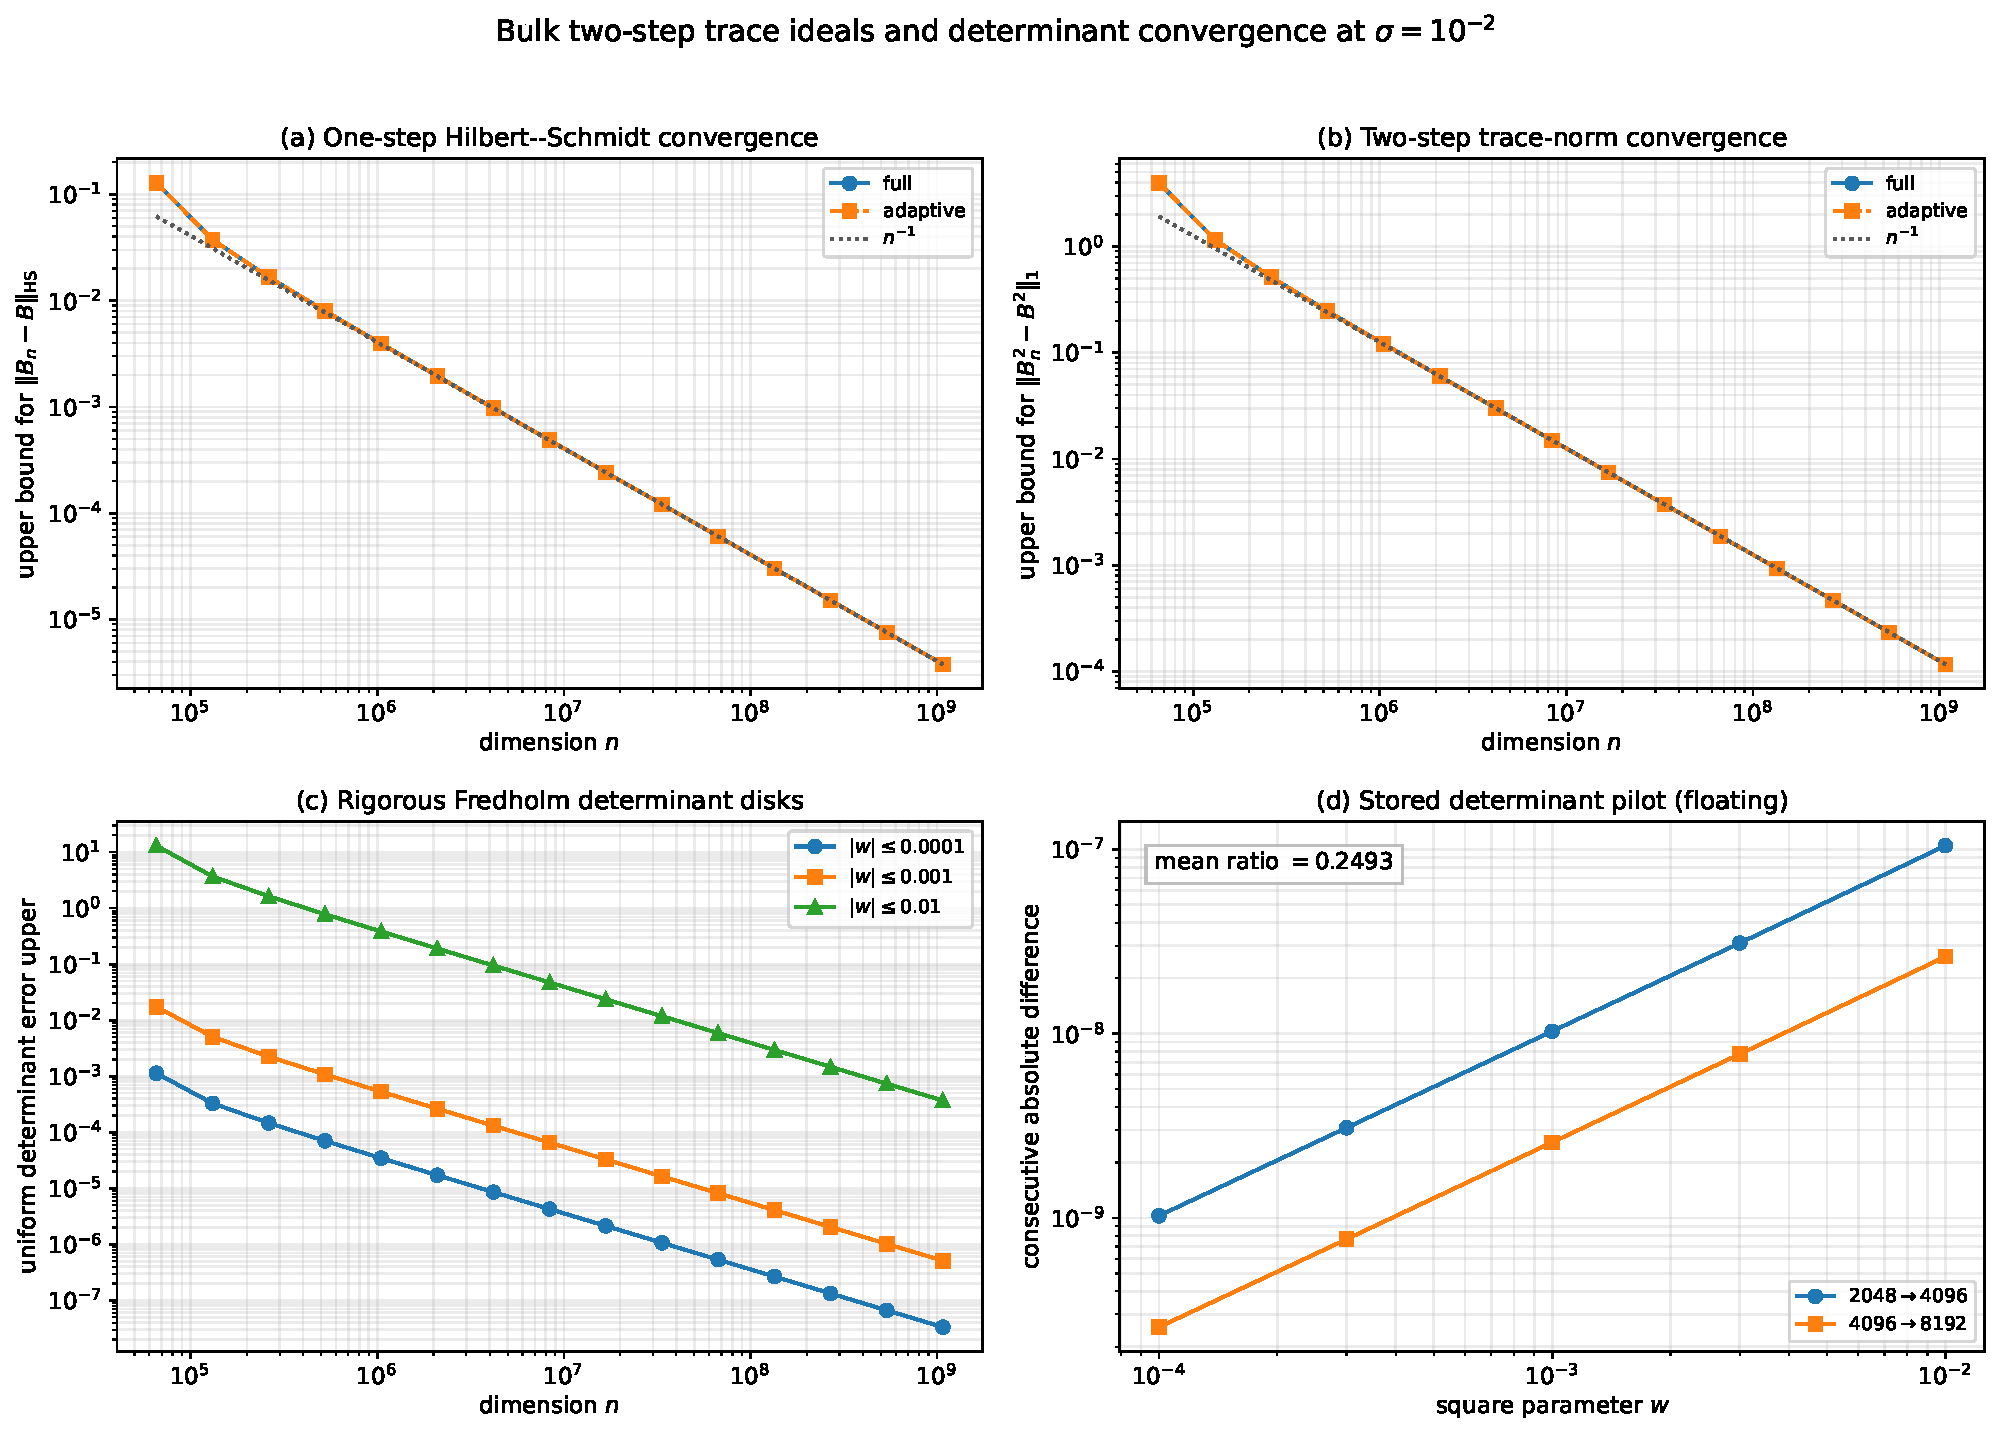
\includegraphics[width=\textwidth]{figures/bulk_two_step_trace_norm_determinant.pdf}
\caption{Trace-ideal completion of the intrinsic bulk.  (a) Outward
Hilbert--Schmidt errors for the full and adaptive one-step bulk families.
(b) The resulting trace-norm errors for their squares.  Both carry the
first-order cellwise Galerkin rate.  (c) Rigorous local-uniform Fredholm
determinant bounds on three $w$-disks.  (d) Floating consecutive differences
of the stored sparse determinants; their approximately quarter scaling is
diagnostic and is not used in panels (a)--(c).}
\label{fig:summary}
\end{figure}

The archive hashes every consumed external certificate, local source,
result, figure, manuscript, and publication PDF.  The complete replay is
listed in the repository README.  Rebuilding the rigorous trace ledger,
tests, figures, and archive takes seconds.  Rebuilding the stored 8192
determinant pilot takes approximately four minutes on the reference server
because each of the five radii requires two sparse LU factorizations.

\section{What is closed and what remains}
\label{sec:boundary}

The present result closes a precise functional-analytic gap.
\begin{enumerate}[leftmargin=2em]
 \item The intrinsic one-step bulk now converges in the natural
 Hilbert--Schmidt topology for full and adaptive discretizations.
 \item Its square converges in trace norm, with a completely explicit
 first-order bound.
 \item Every fixed even bulk trace has a rigorous continuum limit.
 \item The intrinsic two-step Fredholm determinant is the local-uniform
 limit of computable finite determinants.
 \item The determinant is exactly the symmetric product of the two
 regularized one-step determinants from the long-cycle framework.
\end{enumerate}

Several harder bridges remain open.
\begin{enumerate}[leftmargin=2em]
 \item The theorem fixes $\sigma=10^{-2}$.  Uniform trace-ideal control as
 $\sigma\downarrow0$ is not proved.
 \item The fixed eight-sigma family is spectrally stable but is not a
 continuum-convergent family in the norm used here.
 \item No arithmetic formula identifies $\tr(\cB^{2m})$ with a prime or
 prime-power coefficient.
 \item No $T\log T$ zero-counting law has been derived for
 $\cD_{\mathrm{bulk}}$ under any scaling.
 \item The nonnormal operator $\cB$ is not a self-adjoint
 Hilbert--P\'olya operator.  Squaring does not change that fact.
\end{enumerate}

A natural next step is a two-parameter audit: retain the rigorous
trace-ideal topology while allowing the noise width and grid dimension to
vary jointly.  Such a result would determine whether the intrinsic
two-step determinant has a controlled small-noise limit or whether a new
renormalization is required.  Either outcome is mathematically informative.

The current theorem should therefore be read as infrastructure, not as an
arithmetic identification.  It constructs a strict intrinsic cycle-trace
and spectral-determinant object at fixed noise and proves that the archived
finite-dimensional route converges to it in the correct ideal topology.

\section*{Data and code availability}

All source code, outward certificates, stored binary64 inputs, figures,
tests, dependency hashes, archive verification, and the manuscript source
are available in the accompanying repository directory
\url{https://github.com/maris205/prime_dynamics_theory/tree/main/papers/RH-45-bulk-two-step-trace-norm-determinant}.

\bibliographystyle{plainnat}
\bibliography{references}

\end{document}
